\chapter{Background and Theory}


\section{Wireless Sensor Networks}

Sensor networks are collections of small computer that collect sensor data.

\section{RESTful}
\section{HDF}
\section{TDF}

\section{Python}
\section{matplotlib}
\section{scikit-learn}

\section{Supervised Machine Learning Classification algorithms}

Machine learning classification algorithms are used to make decisions based on presented data. For supervised algorithms, data of which the result is known (training data) is used to train a model. Once trained, a model can be presented with unseen data and will automatically decide which class the data falls in to. 

Two standard machine learning algorithms that are used for classification problems, the Support Vector Machine (SVM) and the Aritificial Neural Network (ANN) are discussed in more detail below. 

\subsection{Artificial Neural Networks}
\label{ANNAppendix}

The Artificial Neural Network (ANN) is a machine learning paradigm that attempts to simulate the neurons of the central nervous system of animals and humans. Neural networks in humans and animals are considerably more complicated than ANNs \cite{Graupe2013}; however ANNs attempt to model the way in which real neural networks process information. ANNs can be used for machine learning and pattern recognition, the basic goal is to find a classification result given input data. For example, for recognition of spoken words, the input could be speech audio data and the output could be a number of different words (classes). For a certain speech input, one output word would be chosen. 

In an ANN, neurons are connected together to form a network. The way the neurons are connected is determined by the weight of their connections and this is the basis of the ANN. The weight of connection determines, for each neuron, how important the output of other neurons is. The larger the weight, the more important the connection. Weights can also be negative, which can be thought of as an inhibitive signal \cite{Graupe2013}.

A single neuron may receive inputs from many other neurons. Each input to the neuron is multiplied by the weight of the connection between the receiving and sending neuron. The receiving neuron then computes some mathematical function to determine whether, from the inputs it received, it will activate and send a signal forward. This continues until an output neuron activates which determines which output corresponds to the input given. 

Neurons are typically arranged in layers with only feed-forward connections \cite{Kuan}. The input to the ANN is given to the input layer, which then feeds forward to any number of hidden layers before progressing to an output layer where a classification is made. An example arrangement of neurons can be seen in figure \ref{ANN}. 

\begin{figure}[ht!]
\begin{center}
\leavevmode
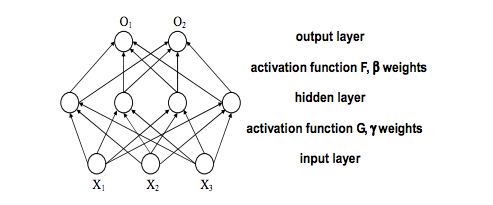
\includegraphics[width=0.5\textwidth]{images/ANN.png}
\end{center}
\caption[Example Artificial Neural Network]{An ANN with 3 input neurons, 4 hidden neurons and 2 output neurons. Figure from Kuan et al. \cite{Kuan}.}
\label{ANN}
\end{figure}

ANN are trained using supervised learning. That is, example input data is given to an ANN where the wanted classification result is known. Using a technique called back propagation, the ANN is progressively updated so that the error for classifying the example data is reduced.  


\subsection{Support Vector Machines}
\label{SVMAppendix}

Support Vector Machines (SVMs) are another machine learning supervised learning technique. Unlike the ANN which can classify input into multiple classes, the SVM only classifies input data into one of two classes. However, it is possible to build  multiple class classification systems using multiple SVMs. 

In training a SVM, the training data consists of input data and the correct binary classification (as there are only two classes that the input data can be classified into).  Using this training data, the SVM then finds the optimal hyperplane or set of hyperplane that best separates the input data of the two classes.  \cite{Jordan2008}

For a set of input data with n dimensions, a n-1 dimension hyperplane will be found. There can be many hyperplanes of this form but for SVMs the best hyperplane is often the hyperplane which maximises the margin between the two classes \cite{Jordan2008}. In this way, the classes are well defined and separated from each other. A simple, two dimensional example of the optimal hyperplane (simply a line in this case) can be seen in figure \ref{SVM}.

\begin{figure}[ht!]
\begin{center}
\leavevmode
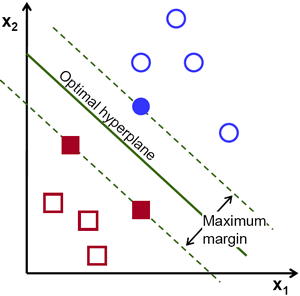
\includegraphics[width=0.5\textwidth]{images/svm.png}
\end{center}
\caption[Example Support Vector Machine]{The optimal hyperplane for a two dimensional example. The two classes are the red circles and blue squares. Figure from OpenCV \cite{SVM}.}
\label{SVM}
\end{figure}

Once trained, the SVM can accept input data and find on which side of the hyperplane the new input data lies. This allows the SVM to classify the data to a particular class. 
\section{Cow eartags}

